\textbf{COLUNI 2020 -- Questão 37}\par\medskip Leia a charge abaixo da cartunista Laerte, publicada em 2011.

% COLUNI-AUTO-FIGURES-BEGIN
\begin{figure}[htbp]
\centering
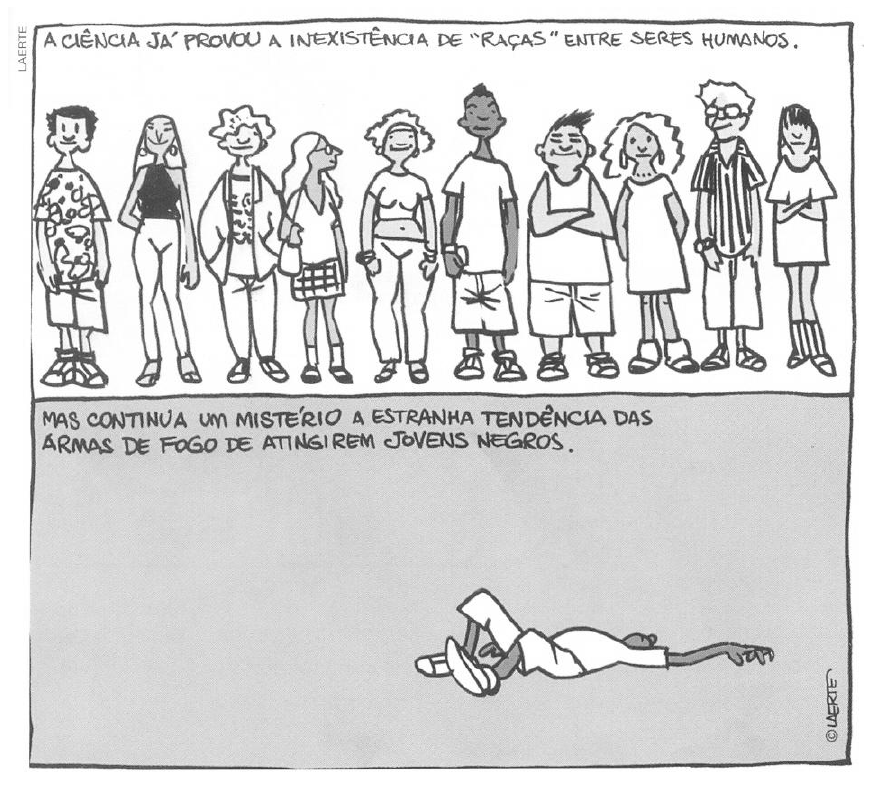
\includegraphics[width=0.95\linewidth]{static/simulados/coluni/figuras/2020/questao-37/figura-1.png}
\end{figure}
% COLUNI-AUTO-FIGURES-END

\par

BRAICK, Patrícia Ramos. \textbf{Estudar História}: das origens do homem à era digital. 2. ed. São Paulo: Moderna, 2015, p. 249.

\par

A respeito de questões suscitadas pela charge sobre a desigualdade racial no Brasil, é INCORRETO afirmar que:

\begin{enumerate}
\item a desigualdade racial no Brasil pode ser verificada em indicadores relacionados à violência urbana, que
        atinge especialmente a população jovem negra.
\item o conjunto de teorias racistas consideradas científicas no contexto da dominação imperialista europeia
        fortaleceu o racismo na sociedade brasileira.
\item as leis sancionadas pelo poder público são instrumentos suficientes para a superação da mentalidade
        racista formada por séculos de escravidão.
\item as ações afirmativas são instrumentos significativos de pressão para a promoção da inclusão
        socioeconômica da população negra no Brasil.\end{enumerate}
